\chapter{ТЕОРЕТИЧЕСКОЕ ОБОСНОВАНИЕ СИСТЕМЫ}
В данной главе рассматриваются модели, которые были рассмотрены при выборе модели системы. Важно отметить, что работа над системой велась с 2011 года. Было выпущено 3 рабочих версии прототипа системы, реализующие различные модели мышления. 
\section{Модели мышления}
В работе было рассмотрено несколько моделей мышления (в скобках кодовое имя прототипа):
\begin{itemize}
	\item Модель мышления Марвина Мински \cite{EmotionMachine} (TU)
	\item Модель мышления на базе нейронных сетей 
	\item Модель с использованием Деревьев Принятия Решений (Menta 0.1)
	\item Модель с использованием Генетических алгоритмов на базе модели мышления Питера Норвига \cite{ArtificialIntelligence} (Menta 0.3)
\end{itemize}



\section{Модель мышления на базе нейронных сетей}
Модель на базе нейронных сетей (поддерживающая обучение) была отброшена на предварительной стадии оценки, так как имеет большие требования производительности \cite{NEURAL} несовместимые с Технико Экономическим Обоснованием \ref{Economic}.


\section{Модель с использованием Деревьев Принятия Решений (Menta 0.1)}
Данная модель являлась одной из первых, которая была опробована. Модель была основана на деревьях принятия решений \cite{DTREE}. В построение модели данной системы использовались следующие компоненты:
\begin{itemize}
	\item Обработка запросов на естественном языке
	\item Поиск решения
	\item Применение решения
\end{itemize}
Системы была ориентирована на выполнение простых команд, например, добавить поле на форму. Основаная функция модели представлена следующим потоком:
\begin{enumerate}
	\item Получение и формализация запроса
	\item Поиск решения при помощи Деревьев Принятия Решений
	\item Изменение модели приложения в формате OWL \cite{OWL}
	\item Генерация и компиляция приложения
\end{enumerate}
Основными проблемами данной модели являлось следующее:
\begin{enumerate}
	\item Отсутствие устойчивости к ошибкам входной информации: грамматическим и содержательным. Например, входной файл не имел отношения к программной системе, модель которой была в базе знаний в формате OWL
	\item Система поиска решения работала только в рамках модели одной программы
	\item Отсутствовала функция обучения 
\end{enumerate}



\section{Модель с использованием Генетических алгоритмов на базе модели мышления Питера Норвига (Menta 0.2-0.3)}
После работы над ошибками была предпринята попытка сделать поиск решения более универсальным. В то время автор работы увлекался генетическими алгоритмами оптимизации и выбор пал на них. В рамках данной модели были сформированы основные компоненты будущей модели:
\begin{itemize}
	\item Критерии Приемки (Acceptance Criteria)
	\item Формат данных OWL 
	\item Использование логических вычислений
\end{itemize}
Система содержала внутри себя модель приложения. При помощи генетического алгоритма модель строила из частей новую систему и проверяла ее при помощи логического движка \cite{NARS} соответствию входным критерия приемки. Основными недостатками подхода оказалось:
\begin{itemize}
	\item Отсутсвие обучения
	\item Отсутсвие обработки естественного языка
\end{itemize}
Кроме того после апробации оказалось, что критерии приемки практически описывают необходимое решение, что являлось недопустимым. Данный подход был описан в статье \cite{SECR}.
\section{Модель мышления Марвина Мински (TU)}
Модель построенная с применением модели мышления Марвина Мински содержала в себе основные концепции предыдущих моделей и показала свою состоятельность на контрольных примерах.
\begin{itemize}
	\item Acceptance Criteria
	\item Обучение
	\item Поиск и применение решения 
	\item Отсутсвие обработки естественного языка
\end{itemize}
Данная модель является более абстрактной и представляется собой верхнеуровневую архитектуру обработки запроса (мышления), где компонентами являются лучшие части предыдущих систем.
\subsection{Крити-Селектор-Путь мышления}
В 2006 году Марвин Мински опубликовал свою книгу "The emotion machine" \cite{EmotionMachine}, в которой предложил свой взгляд на систему мышления и памяти человека. В основу теории легла парадигма триплета Критик-Селектор-Путь мышления, k-line для сопоставления знаний. На рисунке \ref{img:csw} представлена схематичное изображение Критика-Селектора-Пути мышления \\
\begin{figure} [h] 
  \center
  \includegraphics [scale=1.0] {CSW}
  \caption{Критик-Селектор-Путь мышления} 
  \label{img:csw}  
\end{figure}

\textbf{Критик} представляет собой определенный триггер: внешние обстоятельства, события или иное воздействие. Например, включился свет и зрачки сузились. Обожглись и одернули руку. Критик активируется только когда для этого достаточно обстоятельств. Одновременно могут активироваться несколько критиков. Например, человек решает сложную задачу. Идет активация множество критиков: считать, технические детали, кроме того параллельно может активироваться критик переработки, сообщающей о необходимости отдыха.\\
\textbf{Селектор} занимается выбором определенных ресурсов, которыми также являются Пути мышления. \\
\textbf{Путь мышления} это способ решения проблемы. Путь мышления также может активировать следующий критик. \\

На рисунке \ref{img:csw_ex} представления расширенная модель работы триплета Критик-Селектор-Путь мышления. Критик активирует селектор, который активирует путь мышления (синий круг). Путь мышления в свою очередь может активировать критик или же совершить определенные действия. Например, зажегся зеленый свет светофора, значит можно переходить дорогу. \\
Если активировалось много критиков, значит проблему нужно уточнить, так как степень неопределенности слишком высока. Если проблема очень похожа, то можно судить по аналогии.
\begin{figure} [h] 
  \center
  \includegraphics [scale=1.0] {CSW_EX}
  \caption{Критик-Селектор-Путь мышления в разрезе ресурсов} 
  \label{img:csw_ex}  
\end{figure}

\clearpage
\subsection{Уровни мышления}
Концепция уровней мышления представляет собой модель степени ментальной активности человека. Никто из людей не может похвастаться скоростью гепарда, гибкости кошки, силой медведя. Но наш вид все это компенсирует возможностью изобретения путей мышления. Например, чтобы быть быстрыми мы изобрели самолеты, машины. Чтобы быть сильными, мы изобрели оружие. Что же делает это возможным? Безусловно результатом всего является взаимодействие человека с окружающим миром. Именно данное взаимодействие заставляет людей изобретать что-то новое, создавать шедевры литературы и летать в космос. Но как же мы всего этого добиваемся начиная от инстинктивного одергивания руки до создания Теории всего \cite{Hawking}. Далее мы рассмотрим концепцию уровней мышления.
\begin{enumerate}
	\item Инстинктивный уровень
	\item Уровень обученных реакций
	\item Уровень рассуждений
	\item Рефлексивный уровень
	\item Саморефлексивный уровень
	\item Самосознательный уровень
\end{enumerate}

В Таблице \ref{ThinkingLevelDescription} представлено описание уровней мышления.
\begin{table} [htbp]
  \centering
  \parbox{15cm}{\caption{Описание уровней мышления Марвина Мински}\label{ThinkingLevelDescription}}
%  \begin{center}
  \begin{tabular}{| p{5cm} | p{11cm} |}
  \hline
  \hline
Уровень & Описание \\
  \hline
    \hline

Инстинктивный уровень	& На данном уровне происходят инстинктивные реакции (врожденные). Например, боязнь обжечься. Не прыгать под машину. Общую формулу для этого уровня можно выразить как "Если ..., то сделать так". \\
  \hline

Уровень обученных реакций  & На  данной уровне происходит мышление обученных реакций, то есть тех реакций, которыми человек обучается в течение жизни. Например, переходить дорогу на зеленых свет. Общую формулу для этого уровня можно выразить как "Если ..., то сделать так". \\
  \hline

Уровень рассуждений & а  данной уровне происходит мышление с использованием рассуждений. Если я сделаю так, то будет ... Например, если перебежать дорогу на зеленый свет, то можно успеть вовремя. На данном уровне сравниваются последствия нескольких решений и выбирается оптимальное. Общую формулу для этого уровня можно выразить как "Если ..., то сделать так, тогда будет так". \\
  \hline

Рефлексивный уровень  & На данном уровне происходит рассуждение с учетом анализа прошлых событий. Например, прошлый раз я побежал на моргающий зеленый и чуть не попал под машину. \\

  \hline
  Саморефлексивный уровень & На данном уровне происходит оценка себя. Строится определенная модель с помощью которой идет оценка своих поступков. Например, мое решение не пойти на это собрание было неверным, так как я упустил столько возможностей, я был легкомысленный. \\
  \hline
  Самосознательный уровень & Самозонательный уровень на данный момент характерен только для человека. На данном уровне идет оценка поступков человека с точки зрения высших идеалов и внешних оценок. Например, а что подумают мои друзья? А как бы поступил мой герой? \\
  \hline
  
  \end{tabular}
%  \end{center}
\end{table}

Деление на данные уровне носит условный характер. Например уровень 5 и 6 можно объединить. Но по словам Марвина Мински принцип бритвы Оккама успешно применяется в физики, но в психологии он не должен применяться также легко. \\
На рисунке \ref{img:thinkinglevels} представлена схематичное изображение уровней мышления. 1-3 уровни составляют личность человека. 2-5 представляют ЭГО человека (Человеческое Я) - осознание человека в общении с окружающими. 3-6 представляют собой сверх ЭГО человека (сверх Я) - его моральные установки.
\begin{figure} [h] 
  \center
  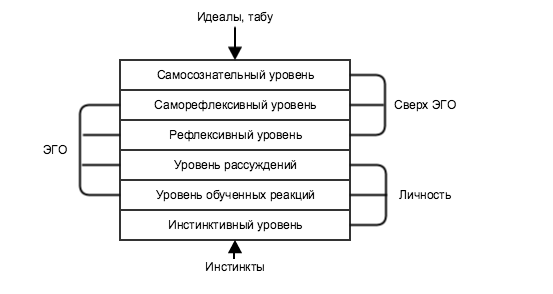
\includegraphics [scale=1.0] {thinkinglevels}
  \caption{Иллюстрация концепции Уровней мышления} 
  \label{img:thinkinglevels}  
\end{figure}
\clearpage
\subsection{K-line}
Концепция K-line была первый раз упомянута Марвином Мински в 1987 году в журнале Cognitive Science. В книге "The Society of Mind" \cite{SocietyOfMind} Марвин Мински раскрывает концепцию K-line. Полностью концепция описана позже в книге "The Emotion Machine" \cite{EmotionMachine}. 
K-line представляет собой связь между двумя событиями, объединяющими их в знание. Например, объединение Пути мышления, найденного решения и активированной проблемы. Данная линия объединяет то как мы думали, решение.
\begin{figure} [h] 
  \center
  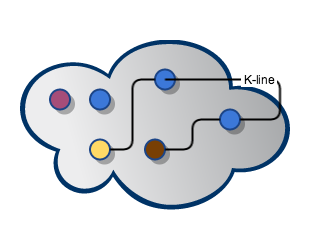
\includegraphics [scale=1.0] {k_line}
  \caption{Иллюстрация концепции K-line} 
  \label{img:k_line}  
\end{figure}
На Рисунке \ref{img:k_line} показана K-line, которая объединяет пути мышления, решение и другие Критики. Данная концепция позволяет "запоминать" удачные решения. 
\clearpage
\section{Выводы по главе}
Для программной экспертной системы очень важно иметь способность мышления и рассуждения. Например, очень важно  для системы уметь действовать по аналогии. Так как множество запросов типичны и отличаются частностями. Например, пожалуйста, установить Office, Antivirus и т.д. \\
Также для экспертной системы важно уметь абстрагировать специализированные рецепты решения. Например, система научилась решать инцидент "Please install Firefox". Абcтрагировав данный инцидент до степени "Please install browser" система сможет теми же способами попробовать решить новый инцидент.\\
После рассмотрения нескольких моделей была выбрана модель мышления Марвина Мински, так как данная модель наиболее точно ложится на целевую область решения инцидентов в области IT. На основе модели мышления Мински была построена модель системы, которая поддерживает основные функции: обучение, понимание инцидента, поиск решения, применение решения. Более подробно с результатами апробации моделей можно ознакомиться на сайте http://tu-project.com


\clearpage